\addcontentsline{toc}{section}{Appendix} % Remove this if you don't want the appendix included in the table of contents.
\appendix

\section{Model Derivations (Part I)}\label{app:part1_derivations}
This section gives the full derivations behind the model equations, coefficients and controller-design formulas used in \Cref{sec:part1}, since the preparation material gives only the result form (e.g.\ ``show that $J_p\ddot p=L_1V_d$'') and not the underlying algebra.

\subsection{Torque balance: $L_1$--$L_4$}\label{app:L_derivation}
\paragraph{Pitch.} The propeller forces $F_b,F_f$ act perpendicular to the pitch arm at distance $l_p$ on either side of the pitch axis, giving a net torque $l_p(F_b-F_f)$. The motor weights $m_pg$ act straight down at the same distance $l_p$ on either side and are equal in magnitude, so their torques cancel exactly regardless of $p$; gravity therefore does not appear in the pitch equation. Hence
\begin{equation}
	J_p\ddot p = l_p(F_b-F_f) = l_pK_f(V_b-V_f) = l_pK_fV_d \;\Rightarrow\; L_1=l_pK_f.
\end{equation}

\paragraph{Elevation.} The counterweight and motor weights are vertical, but the elevation arm is tilted by $e$, so their moment arm is the horizontal projection of the arm, i.e.\ scaled by $\cos(e)$:
\begin{equation}
	\tau_{\text{gravity}} = g(m_cl_c-2m_pl_h)\cos(e).
\end{equation}
The propeller thrust $F_b+F_f$ is itself tilted by the pitch angle $p$; only its component along the elevation direction, scaled by $\cos(p)$, contributes, acting at distance $l_h$:
\begin{equation}
	\tau_{\text{propeller}} = l_h(F_b+F_f)\cos(p) = l_hK_fV_s\cos(p).
\end{equation}
Summing gives $J_e\ddot e = g(m_cl_c-2m_pl_h)\cos(e) + l_hK_fV_s\cos(p)$, hence $L_2=g(m_cl_c-2m_pl_h)$ and $L_3=l_hK_f$.

\paragraph{Travel.} Only the component of the propeller thrust perpendicular to the arm's projection contributes to travel, i.e.\ the $\sin(p)$-component, acting at horizontal distance $l_h\cos(e)$ from the travel axis:
\begin{equation}
	J_\lambda\ddot\lambda = l_h\cos(e)(F_b+F_f)\sin(p) = l_hK_fV_s\cos(e)\sin(p) \;\Rightarrow\; L_4=l_hK_f=L_3,
\end{equation}
i.e.\ $L_3$ and $L_4$ share the same physical origin (the propeller thrust acting at arm $l_h$), hence $L_3=L_4$.

\subsection{Linearisation about $p=e=0$: $K_1,K_2,K_3$ and $V_{s,0}$}\label{app:K_derivation}
The pitch equation $J_p\ddot p=L_1V_d$ is already linear, giving $K_1=L_1/J_p$ directly.

For elevation, write $f(e,p,V_s)=L_2\cos(e)+L_3V_s\cos(p)$ and Taylor-expand about $(e,p,V_s)=(0,0,V_{s,0})$:
\begin{equation}
	f \approx f(0,0,V_{s,0}) + \frac{\partial f}{\partial e}\bigg|_0 e + \frac{\partial f}{\partial p}\bigg|_0 p + \frac{\partial f}{\partial V_s}\bigg|_0(V_s-V_{s,0}).
\end{equation}
Since $\partial f/\partial e=-L_2\sin(e)\to0$ and $\partial f/\partial p=-L_3V_s\sin(p)\to0$ at $(0,0)$, while $\partial f/\partial V_s=L_3\cos(p)\to L_3$, this reduces to
\begin{equation}
	f \approx (L_2+L_3V_{s,0}) + L_3\tilde V_s, \qquad \tilde V_s := V_s - V_{s,0}.
\end{equation}
For $(p,e)=(0,0)$ to be a genuine equilibrium, the constant term must vanish when $\tilde V_s=0$, i.e.
\begin{equation}
	L_2 + L_3V_{s,0} = 0 \;\Rightarrow\; V_{s,0} = -L_2/L_3.
\end{equation}
With this condition, $J_e\ddot e \approx L_3\tilde V_s$, giving $K_2=L_3/J_e$.

For travel, write $g(e,p,V_s)=L_4V_s\cos(e)\sin(p)$. At $(0,0,V_{s,0})$: $g=0$, and both $\partial g/\partial e$ and $\partial g/\partial V_s$ contain a factor $\sin(p)\to0$, so only $\partial g/\partial p=L_4V_s\cos(e)\cos(p)\to L_4V_{s,0}$ survives:
\begin{equation}
	J_\lambda\ddot\lambda \approx L_4V_{s,0}\,p \;\Rightarrow\; K_3 = L_4V_{s,0}/J_\lambda.
\end{equation}
Substituting $L_4=L_3$ and $V_{s,0}=-L_2/L_3$ gives $K_3=-L_2/J_\lambda$, independent of $K_f$ (which cancels along with $L_3$).

\subsection{Solving for $K_f$}\label{app:Kf_derivation}
From $V_{s,0}=-L_2/L_3=-L_2/(l_hK_f)$, solving for $K_f$ gives
\begin{equation}
	K_f = -\frac{L_2}{l_hV_{s,0}},
\end{equation}
the only constant here that is not pure algebra: $V_{s,0}$ is measured experimentally in Task~2 and substituted in.

\subsection{Closed-loop transfer function $G(s)$}\label{app:G_derivation}
Substituting the PD control law $V_d=K_{pp}(p_c-p)-K_{pd}\dot p$ into $\ddot p=K_1V_d$ gives
\begin{equation}
	\ddot p + K_1K_{pd}\dot p + K_1K_{pp}p = K_1K_{pp}p_c.
\end{equation}
Taking the Laplace transform with zero initial conditions,
\begin{equation}
	s^2P(s) + K_1K_{pd}\,sP(s) + K_1K_{pp}P(s) = K_1K_{pp}P_c(s),
\end{equation}
so
\begin{equation}
	G(s) = \frac{P(s)}{P_c(s)} = \frac{K_1K_{pp}}{s^2+K_1K_{pd}s+K_1K_{pp}} =: \frac{K_1K_{pp}}{D(s)}.
\end{equation}

\subsection{Pole placement: $\lambda_1,\lambda_2$ versus $\zeta,\omega_0$}\label{app:pole_derivation}
Matching $D(s)$ against the desired poles, $D(s)=(s-\lambda_1)(s-\lambda_2)=s^2-(\lambda_1+\lambda_2)s+\lambda_1\lambda_2$, and comparing coefficients with $D(s)=s^2+K_1K_{pd}s+K_1K_{pp}$ gives
\begin{equation}\label{eq:kpp_kpd_lambda}
	K_{pd} = -\frac{\lambda_1+\lambda_2}{K_1}, \qquad K_{pp} = \frac{\lambda_1\lambda_2}{K_1}.
\end{equation}
Alternatively, comparing $D(s)$ with the standard second-order polynomial $s^2+2\zeta\omega_0s+\omega_0^2$ term by term gives $K_1K_{pp}=\omega_0^2$ and $K_1K_{pd}=2\zeta\omega_0$, i.e.\ \Cref{eq:kpp_kpd_zeta} in \Cref{sec:prob_descr}, which is what \texttt{init\_heli\_3\_10.m} implements. The two parametrisations are related by $\lambda_{1,2}=-\zeta\omega_0\pm\omega_0\sqrt{\zeta^2-1}$.

We prefer $(\zeta,\omega_0)$ over specifying $\lambda_1,\lambda_2$ directly for three reasons. First, $\lambda_1,\lambda_2$ are only real for $\zeta\geq1$; every underdamped case in our test-plan (\Cref{sec:part1_testplan}) has a complex-conjugate pole pair, so choosing $\lambda_{1,2}$ directly would mean specifying a complex number by hand for most tests, whereas $(\zeta,\omega_0)$ are two real numbers that sweep continuously from underdamped through critically damped to overdamped without special-casing. Second, $\zeta$ and $\omega_0$ separate \emph{how oscillatory} the response is from \emph{how fast} it is, connecting directly to the standard second-order step-response quantities (overshoot, settling time) that the assignment asks us to hypothesise about; $\lambda_1,\lambda_2$ affect $K_{pp}$ and $K_{pd}$ jointly through their sum and product, which is far less intuitive to reason about before a test. Third, allowing $\zeta<0$ is a deliberate, single-parameter way to place a pole in the right half-plane and produce a controlled instability, which we use in Task~3 to probe the boundary between theory and the physical (saturating) system.

\section{MATLAB Code}\label{sec:matlab}
This section should contain your MATLAB code. DO NOT attach files posted online (that you didn't write). Note that the method used to input code below does not look as pretty when the lines are too long.

\subsection{plot\_constraint.m}\label{sec:plot_constraint_m}
\lstinputlisting{code/plot_constraint.m}\section{Simulink Diagrams}\label{sec:simulink}
This section should contain your Simulink diagrams. Just like the plots, these should be in vector format, like in \Cref{fig:simulink}. Make them tidy enough to understand.

\subsection{A Simulink Diagram}
\Cref{fig:simulink} shows a Simulink diagram. You can use the \texttt{print\_simulink.m} function, included in the source code repository for this document, to export a Simulink model to EPS\@.
\begin{figure}[htb]
	\centering
		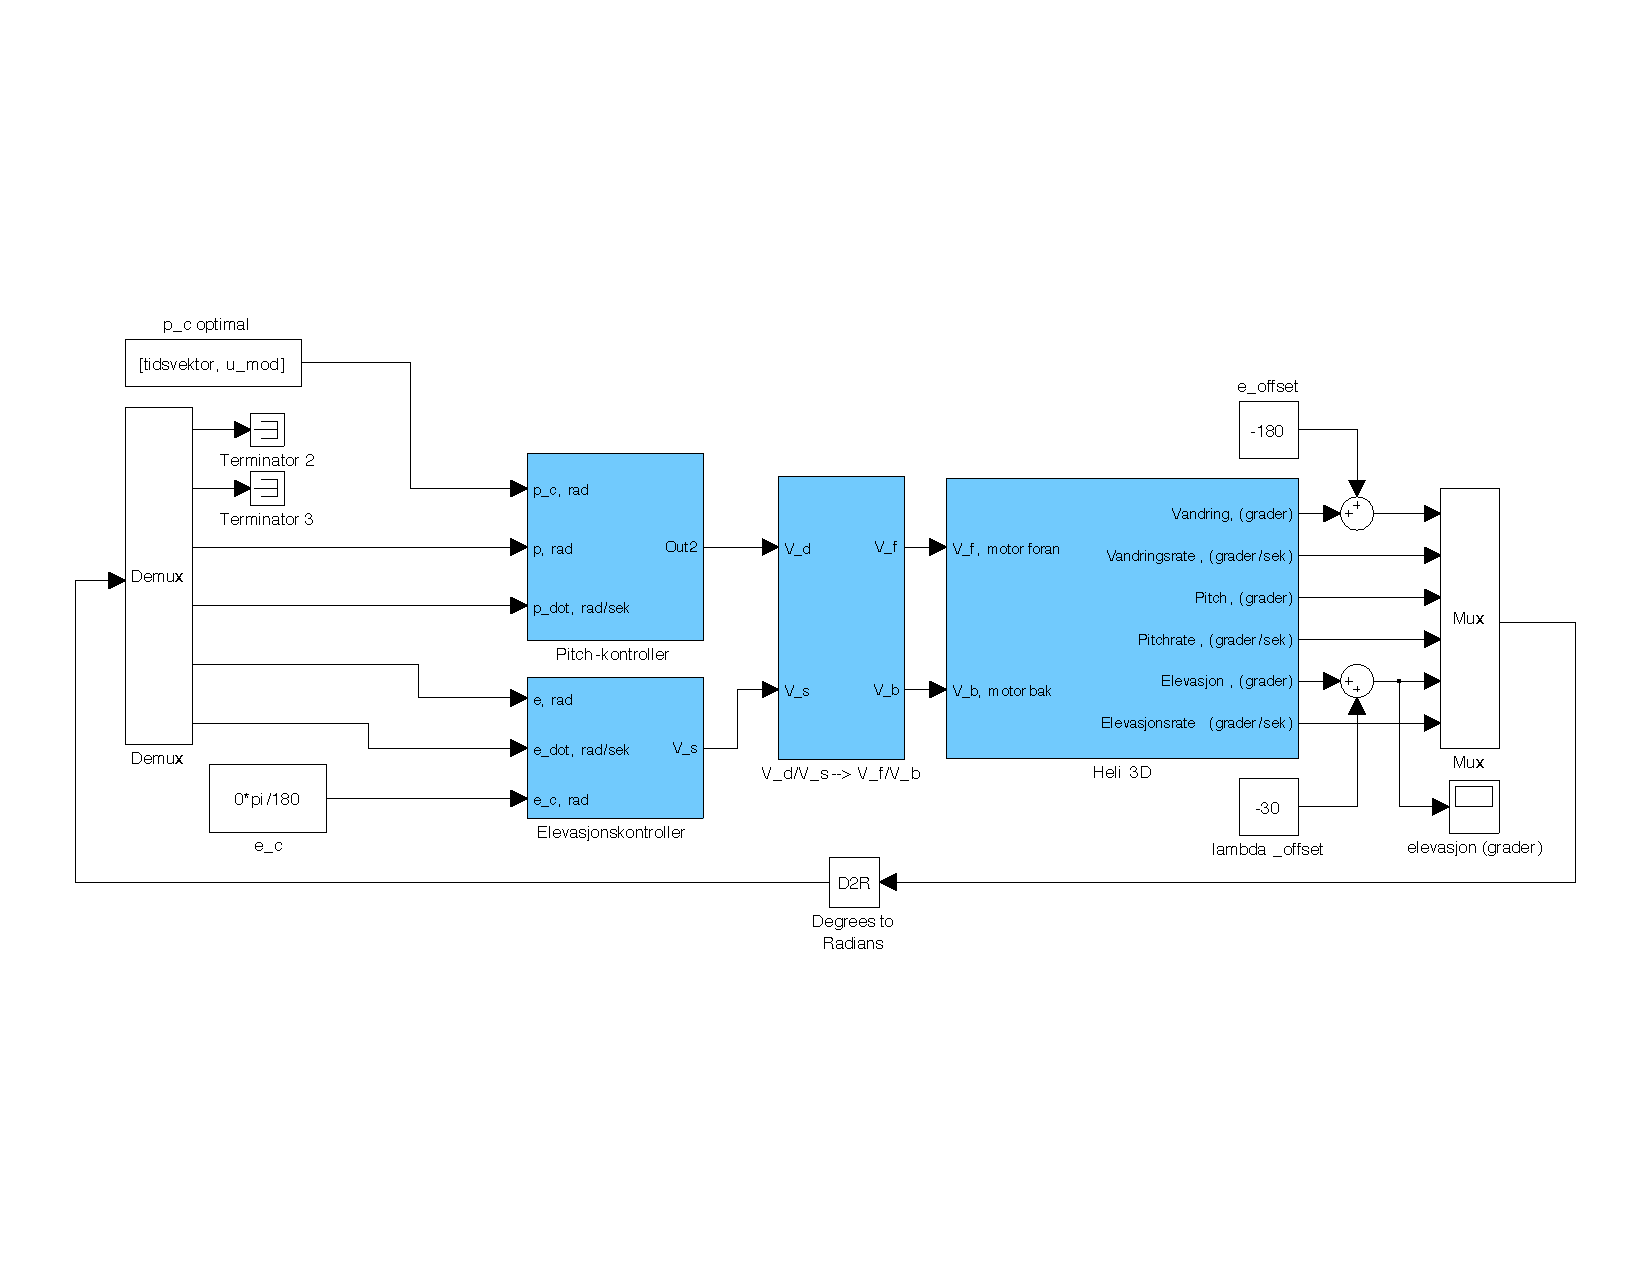
\includegraphics[width = \textwidth]{figures/simulink.pdf}
	\caption{A Simulink diagram.}
\label{fig:simulink}
\end{figure}
